\documentclass[supercite]{Experimental_Report}

\title{~~~~~~新生实践课~~~~~~}
\author{彭嘉炜}
\school{计算机科学与技术学院}
\classnum{CS2110}
\stunum{U202115630}
\instructor{陈加忠} % 李平、孙伟平、范晔斌、陈加忠
\date{2021年11月11日}
\usepackage{zhnumber} % change section number to chinese
\renewcommand\thesection{\zhnum{section}}
\renewcommand \thesubsection {\arabic{subsection}}
\usepackage{algorithm, multirow}
\usepackage{algpseudocode}
\usepackage{amsmath}
\usepackage{amsthm}
\usepackage{framed}
\usepackage{mathtools}
\usepackage{subcaption}
\usepackage{xltxtra} %提供了针对XeTeX的改进并且加入了XeTeX的LOGO, 自动调用xunicode宏包(提供Unicode字符宏)
\usepackage{bm}
\usepackage{tikz}
\usepackage{tikzscale}
\usepackage{pgfplots}
%\usepackage{enumerate}

\pgfplotsset{compat=1.16}

\newcommand{\cfig}[3]{
  \begin{figure}[htb]
    \centering
    \includegraphics[width=#2\textwidth]{images/#1.tikz}
    \caption{#3}
    \label{fig:#1}
  \end{figure}
}

\newcommand{\sfig}[3]{
  \begin{subfigure}[b]{#2\textwidth}
    \includegraphics[width=\textwidth]{images/#1.tikz}
    \caption{#3}
    \label{fig:#1}
  \end{subfigure}
}

\newcommand{\xfig}[3]{
  \begin{figure}[htb]
    \centering
    #3
    \caption{#2}
    \label{fig:#1}
  \end{figure}
}

\newcommand{\rfig}[1]{\autoref{fig:#1}}
\newcommand{\ralg}[1]{\autoref{alg:#1}}
\newcommand{\rthm}[1]{\autoref{thm:#1}}
\newcommand{\rlem}[1]{\autoref{lem:#1}}
\newcommand{\reqn}[1]{\autoref{eqn:#1}}
\newcommand{\rtbl}[1]{\autoref{tbl:#1}}

\algnewcommand\Null{\textsc{null }}
\algnewcommand\algorithmicinput{\textbf{Input:}}
\algnewcommand\Input{\item[\algorithmicinput]}
\algnewcommand\algorithmicoutput{\textbf{Output:}}
\algnewcommand\Output{\item[\algorithmicoutput]}
\algnewcommand\algorithmicbreak{\textbf{break}}
\algnewcommand\Break{\algorithmicbreak}
\algnewcommand\algorithmiccontinue{\textbf{continue}}
\algnewcommand\Continue{\algorithmiccontinue}
\algnewcommand{\LeftCom}[1]{\State $\triangleright$ #1}

\newtheorem{thm}{定理}[section]
\newtheorem{lem}{引理}[section]

\colorlet{shadecolor}{black!15}

\theoremstyle{definition}
\newtheorem{alg}{算法}[section]

\def\thmautorefname~#1\null{定理~#1~\null}
\def\lemautorefname~#1\null{引理~#1~\null}
\def\algautorefname~#1\null{算法~#1~\null}

\begin{document}

\maketitle

\clearpage

\pagenumbering{Roman}

%\tableofcontents[level=2]

\pagenumbering{arabic}

\section{网页整体框架}

图\ref{fig1-1}只是网页整体框架举例,它是用visio画的,然后再在visio里通过文件-打印,如图\ref{fig1-2}所示打印成pdf文件,然后再用pdf阅览器的工具,如图\ref{fig1-3}所示,做适当的裁剪。画图说明网页的整体框架,进行简要的文字描述等。画图说明网页的整体框架,进行简要的文字描述等。画图说明网页的整体框架,进行简要的文字描述等。画图说明网页的整体框架,进行简要的文字描述等。画图说明网页的整体框架,进行简要的文字描述等。画图说明网页的整体框架,进行简要的文字描述等。画图说明网页的整体框架,进行简要的文字描述等。

\begin{enumerate}
\renewcommand{\labelenumi}{\theenumi)}
	\item C++
	\item Java
	\item HTML
\end{enumerate}

画图说明网页的整体框架,进行简要的文字描述等。画图说明网页的整体框架,进行简要的文字描述等。画图说明网页的整体框架,进行简要的文字描述等。画图说明网页的整体框架,进行简要的文字描述等。画图说明网页的整体框架,进行简要的文字描述等。画图说明网页的整体框架,进行简要的文字描述等。画图说明网页的整体框架,进行简要的文字描述等。

画图说明网页的整体框架,进行简要的文字描述等。画图说明网页的整体框架,进行简要的文字描述等。画图说明网页的整体框架,进行简要的文字描述等。画图说明网页的整体框架,进行简要的文字描述等。画图说明网页的整体框架,进行简要的文字描述等。画图说明网页的整体框架,进行简要的文字描述等。画图说明网页的整体框架,进行简要的文字描述等。

画图说明网页的整体框架,进行简要的文字描述等。画图说明网页的整体框架,进行简要的文字描述等。画图说明网页的整体框架,进行简要的文字描述等。画图说明网页的整体框架,进行简要的文字描述等。画图说明网页的整体框架,进行简要的文字描述等。画图说明网页的整体框架,进行简要的文字描述等。画图说明网页的整体框架,进行简要的文字描述等。

画图说明网页的整体框架,进行简要的文字描述等。画图说明网页的整体框架,进行简要的文字描述等。画图说明网页的整体框架,进行简要的文字描述等。画图说明网页的整体框架,进行简要的文字描述等。画图说明网页的整体框架,进行简要的文字描述等。画图说明网页的整体框架,进行简要的文字描述等。画图说明网页的整体框架,进行简要的文字描述等。

\begin{figure}[htb] % here top bottom
	\begin{center}
		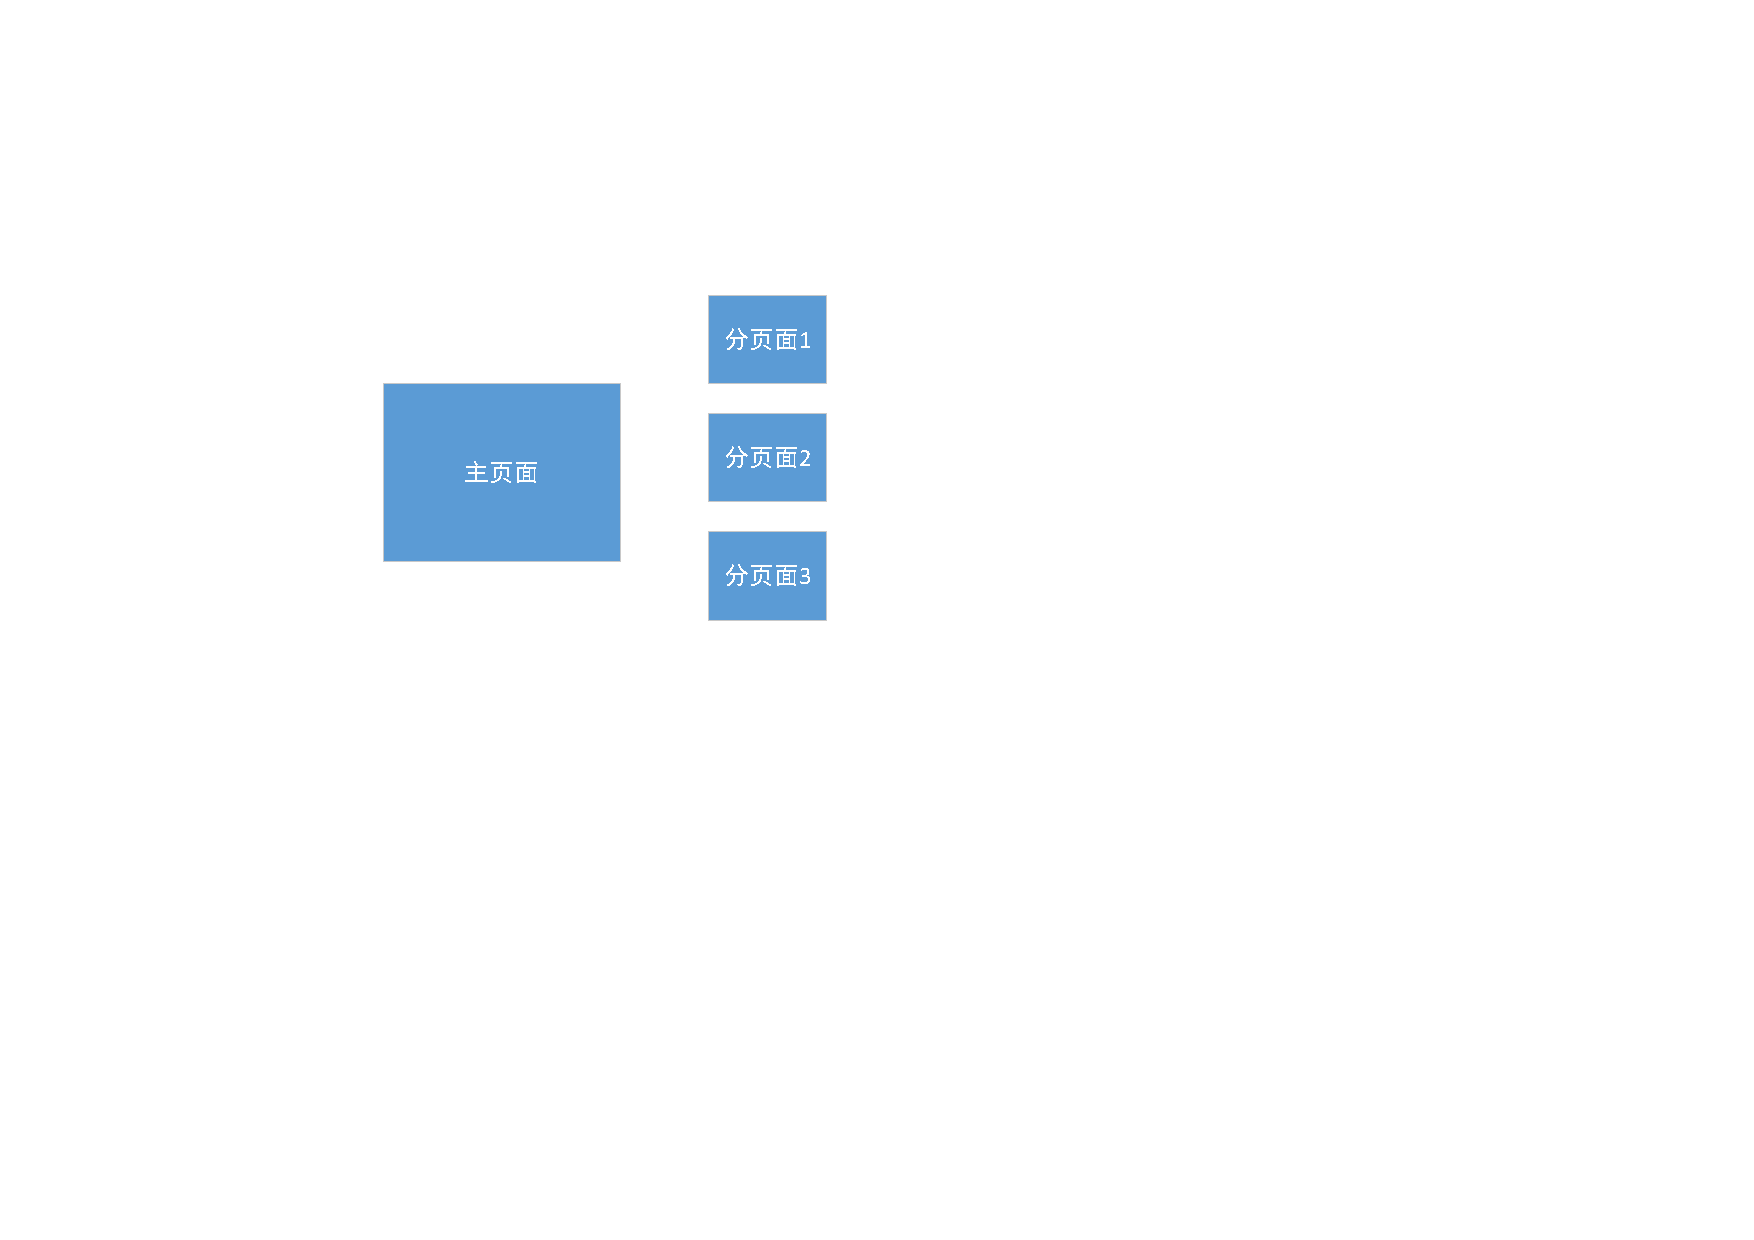
\includegraphics[scale=0.80]{images/1-1.pdf}
		\caption{网页整体框架举例}
		\label{fig1-1}
	\end{center}
\end{figure}

画图说明网页的整体框架,进行简要的文字描述等。画图说明网页的整体框架,进行简要的文字描述等。画图说明网页的整体框架,进行简要的文字描述等。画图说明网页的整体框架,进行简要的文字描述等。画图说明网页的整体框架,进行简要的文字描述等。画图说明网页的整体框架,进行简要的文字描述等。画图说明网页的整体框架,进行简要的文字描述等。

\begin{figure}[htb]
	\begin{center}
		
\includegraphics[scale=0.60]{images/1-2.png}
		\caption{在visio里通过文件-打印,把visio图打印成pdf文件}
		\label{fig1-2}
	\end{center}
\end{figure}

画图说明网页的整体框架,进行简要的文字描述等。画图说明网页的整体框架,进行简要的文字描述等。画图说明网页的整体框架,进行简要的文字描述等。画图说明网页的整体框架,进行简要的文字描述等。画图说明网页的整体框架,进行简要的文字描述等。画图说明网页的整体框架,进行简要的文字描述等。画图说明网页的整体框架,进行简要的文字描述等。

\begin{figure}[htb]
	\begin{center}
		
\includegraphics[scale=0.50]{images/1-3.png}
		\caption{用pdf阅览器的工具,对打印得到pdf图做适当的裁剪}
		\label{fig1-3}
	\end{center}
\end{figure}

画图说明网页的整体框架,进行简要的文字描述等。画图说明网页的整体框架,进行简要的文字描述等。画图说明网页的整体框架,进行简要的文字描述等。画图说明网页的整体框架,进行简要的文字描述等。画图说明网页的整体框架,进行简要的文字描述等。画图说明网页的整体框架,进行简要的文字描述等。画图说明网页的整体框架,进行简要的文字描述等。

\newpage

\section{主页设计}

描述主页的结构,给出主页截图,描述主要设计思路等,请见图\ref{fig2-1}。描述主页的结构,给出主页截图,描述主要设计思路等。描述主页的结构,给出主页截图,描述主要设计思路等。描述主页的结构,给出主页截图,描述主要设计思路等。描述主页的结构,给出主页截图,描述主要设计思路等。描述主页的结构,给出主页截图,描述主要设计思路等。描述主页的结构,给出主页截图,描述主要设计思路等。

\begin{figure}[htb]
	\begin{center}
		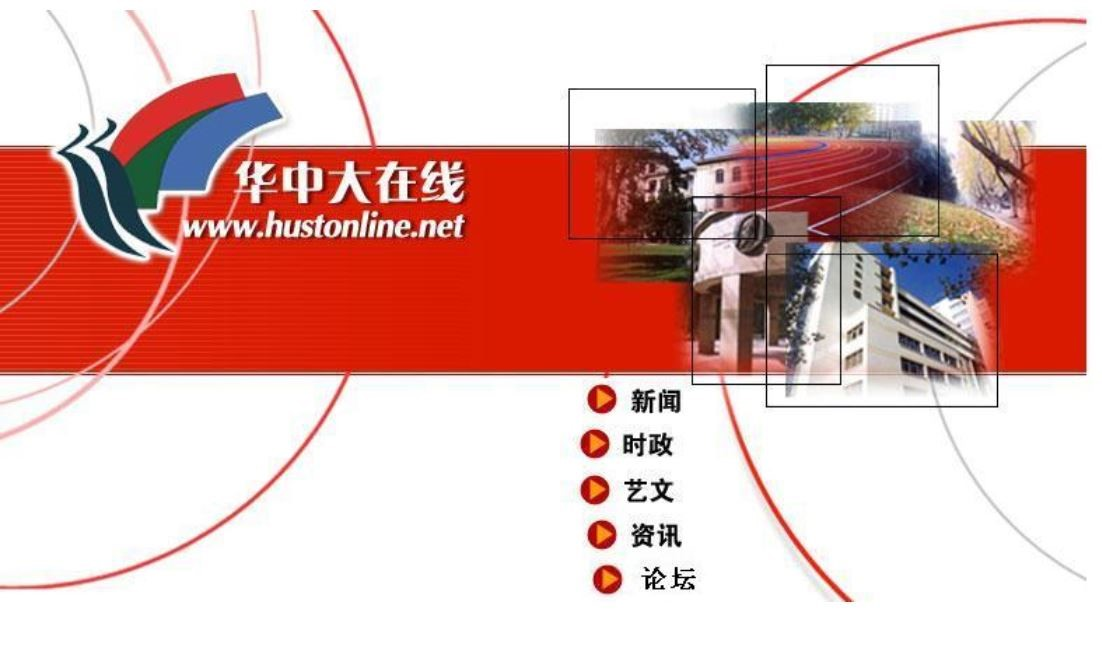
\includegraphics[scale=0.40]{images/2-1.jpg}
		\caption{主页举例}
		\label{fig2-1}
	\end{center}
\end{figure}

描述主页的结构,给出主页截图,描述主要设计思路等。描述主页的结构,给出主页截图,描述主要设计思路等。描述主页的结构,给出主页截图,描述主要设计思路等。描述主页的结构,给出主页截图,描述主要设计思路等。描述主页的结构,给出主页截图,描述主要设计思路等。描述主页的结构,给出主页截图,描述主要设计思路等。描述主页的结构,给出主页截图,描述主要设计思路等。

描述主页的结构,给出主页截图,描述主要设计思路等。描述主页的结构,给出主页截图,描述主要设计思路等。描述主页的结构,给出主页截图,描述主要设计思路等。描述主页的结构,给出主页截图,描述主要设计思路等。描述主页的结构,给出主页截图,描述主要设计思路等。描述主页的结构,给出主页截图,描述主要设计思路等。描述主页的结构,给出主页截图,描述主要设计思路等。

描述主页的结构,给出主页截图,描述主要设计思路等。描述主页的结构,给出主页截图,描述主要设计思路等。描述主页的结构,给出主页截图,描述主要设计思路等。描述主页的结构,给出主页截图,描述主要设计思路等。描述主页的结构,给出主页截图,描述主要设计思路等。描述主页的结构,给出主页截图,描述主要设计思路等。描述主页的结构,给出主页截图,描述主要设计思路等。

描述主页的结构,给出主页截图,描述主要设计思路等。描述主页的结构,给出主页截图,描述主要设计思路等。描述主页的结构,给出主页截图,描述主要设计思路等。描述主页的结构,给出主页截图,描述主要设计思路等。描述主页的结构,给出主页截图,描述主要设计思路等。描述主页的结构,给出主页截图,描述主要设计思路等。描述主页的结构,给出主页截图。

\newpage

\section{分页面设计}

给出分页面截图,描述主要设计思路等。给出分页面截图,描述主要设计思路等。给出分页面截图,描述主要设计思路等。给出分页面截图,描述主要设计思路等。

\subsection{页面1 (每个页面以主要内容起标题名称即可)}

给出分页面截图,描述主要设计思路等。给出分页面截图,描述主要设计思路等。给出分页面截图,描述主要设计思路等。给出分页面截图,描述主要设计思路等。给出分页面截图,描述主要设计思路等。给出分页面截图,描述主要设计思路等。给出分页面截图,描述主要设计思路等。给出分页面截图,描述主要设计思路等。给出分页面截图,描述主要设计思路等。给出分页面截图,描述主要设计思路等。给出分页面截图,描述主要设计思路等。给出分页面截图,描述主要设计思路等。给出分页面截图,描述主要设计思路等。

如果实验报告中要用到算法伪代码,请参考算法\ref{alg:1},也可以参考算法\ref{alg:2}。如果实验报告中要用到算法伪代码,请参考算法\ref{alg:1},也可以参考算法\ref{alg:2}。如果实验报告中要用到算法伪代码,请参考算法\ref{alg:1},也可以参考算法\ref{alg:2}。如果实验报告中要用到算法伪代码,请参考算法\ref{alg:1},也可以参考算法\ref{alg:2}。

\begin{shaded*}\begin{alg}{一个复杂算法}
		\label{alg:1}
		\begin{algorithmic}
			\Input Two numbers $a$ and $b$
			\Output The sum of $a$ and $b$
			\Procedure{A-Plus-B}{$a, b$}
			\If $a = 0$
			\State \Return $b$
			\EndIf
			\State $res \gets 0$
			\While{$b \neq 0$}
			\State Increase $res$ by $1$
			\State $b \gets b - 1$
			\EndWhile
			\State \Return $res$
			\EndProcedure
		\end{algorithmic}
\end{alg}\end{shaded*}

\subsection{页面2 (每个页面以主要内容起标题名称即可)}

给出分页面截图,描述主要设计思路等。给出分页面截图,描述主要设计思路等。给出分页面截图,描述主要设计思路等。给出分页面截图,描述主要设计思路等。给出分页面截图,描述主要设计思路等。给出分页面截图,描述主要设计思路等。给出分页面截图,描述主要设计思路等。给出分页面截图,描述主要设计思路等。给出分页面截图,描述主要设计思路等。给出分页面截图,描述主要设计思路等。给出分页面截图,描述主要设计思路等。


如果实验报告中要用到算法伪代码,请参考算法\ref{alg:1},也可以参考算法\ref{alg:2}。如果实验报告中要用到算法伪代码,请参考算法\ref{alg:1},也可以参考算法\ref{alg:2}。如果实验报告中要用到算法伪代码,请参考算法\ref{alg:1},也可以参考算法\ref{alg:2}。如果实验报告中要用到算法伪代码,请参考算法\ref{alg:1},也可以参考算法\ref{alg:2}。

\begin{algorithm}[h] 
	\caption{一个更复杂算法}
	\begin{algorithmic}[1]
		\State Initialization: $I_{xy}$, $z_{f}=Zeros(128, 128)$; 
		\For{$0\leq n \textless N$}
		\State $i=\lfloor x_n \rfloor+64$, $j=\lfloor y_n \rfloor + 64$
		\If{$z_n<0$ and $|z_n|>|z_{f}(i,j)|$};
		\State $z_{f}(i,j)=z_n$;
		\EndIf
		\State $I_{xy}(i,j)=z_{f}(i,j)$;
		\EndFor 
	\end{algorithmic}\label{alg:2}
\end{algorithm}

\subsection{页面3 (每个页面以主要内容起标题名称即可)}

给出分页面截图,描述主要设计思路等。给出分页面截图,描述主要设计思路等。给出分页面截图,描述主要设计思路等。给出分页面截图,描述主要设计思路等。给出分页面截图,描述主要设计思路等。给出分页面截图,描述主要设计思路等。给出分页面截图,描述主要设计思路等。给出分页面截图,描述主要设计思路等。给出分页面截图,描述主要设计思路等。给出分页面截图,描述主要设计思路等。给出分页面截图,描述主要设计思路等。

\subsection{页面4 (每个页面以主要内容起标题名称即可)}

给出分页面截图,描述主要设计思路等。给出分页面截图,描述主要设计思路等。给出分页面截图,描述主要设计思路等。给出分页面截图,描述主要设计思路等。给出分页面截图,描述主要设计思路等。给出分页面截图,描述主要设计思路等。给出分页面截图,描述主要设计思路等。给出分页面截图,描述主要设计思路等。给出分页面截图,描述主要设计思路等。给出分页面截图,描述主要设计思路等。给出分页面截图,描述主要设计思路等。

\newpage

\section{网页设计小结}

描述网页的设计和实现过程中遇到的问题及如何解决。描述网页的设计和实现过程中遇到的问题及如何解决。描述网页的设计和实现过程中遇到的问题及如何解决。描述网页的设计和实现过程中遇到的问题及如何解决。描述网页的设计和实现过程中遇到的问题及如何解决。描述网页的设计和实现过程中遇到的问题及如何解决。描述网页的设计和实现过程中遇到的问题及如何解决。描述网页的设计和实现过程中遇到的问题及如何解决。描述网页的设计和实现过程中遇到的问题及如何解决。

描述网页的设计和实现过程中遇到的问题及如何解决。描述网页的设计和实现过程中遇到的问题及如何解决。描述网页的设计和实现过程中遇到的问题及如何解决。描述网页的设计和实现过程中遇到的问题及如何解决。描述网页的设计和实现过程中遇到的问题及如何解决。描述网页的设计和实现过程中遇到的问题及如何解决。描述网页的设计和实现过程中遇到的问题及如何解决。描述网页的设计和实现过程中遇到的问题及如何解决。描述网页的设计和实现过程中遇到的问题及如何解决。

描述网页的设计和实现过程中遇到的问题及如何解决。描述网页的设计和实现过程中遇到的问题及如何解决。描述网页的设计和实现过程中遇到的问题及如何解决。描述网页的设计和实现过程中遇到的问题及如何解决。描述网页的设计和实现过程中遇到的问题及如何解决。描述网页的设计和实现过程中遇到的问题及如何解决。描述网页的设计和实现过程中遇到的问题及如何解决。描述网页的设计和实现过程中遇到的问题及如何解决。描述网页的设计和实现过程中遇到的问题及如何解决。

描述网页的设计和实现过程中遇到的问题及如何解决。描述网页的设计和实现过程中遇到的问题及如何解决。描述网页的设计和实现过程中遇到的问题及如何解决。描述网页的设计和实现过程中遇到的问题及如何解决。描述网页的设计和实现过程中遇到的问题及如何解决。描述网页的设计和实现过程中遇到的问题及如何解决。描述网页的设计和实现过程中遇到的问题及如何解决。描述网页的设计和实现过程中遇到的问题及如何解决。描述网页的设计和实现过程中遇到的问题及如何解决。

\newpage

\section{课程的收获和建议}

描述通过学习该专题,有何收获,有何建议,如某专题可适当减少讲授时间、某专题可适当增加讲授内容和时间等。描述通过学习该专题,有何收获,有何建议,如某专题可适当减少讲授时间、某专题可适当增加讲授内容和时间等。描述通过学习该专题,有何收获,有何建议,如某专题可适当减少讲授时间、某专题可适当增加讲授内容和时间等。描述通过学习该专题,有何收获,有何建议,如某专题可适当减少讲授时间、某专题可适当增加讲授内容和时间等。

\subsection{计算机基础知识}

描述通过学习计算机基础知识专题,有何收获,有何建议,如某专题可适当减少讲授时间、某专题可适当增加讲授内容和时间等。描述网页的设计和实现过程中遇到的问题及如何解决。描述网页的设计和实现过程中遇到的问题及如何解决。描述网页的设计和实现过程中遇到的问题及如何解决。描述网页的设计和实现过程中遇到的问题及如何解决。描述网页的设计和实现过程中遇到的问题及如何解决。描述网页的设计和实现过程中遇到的问题及如何解决。描述网页的设计和实现过程中遇到的问题及如何解决。描述网页的设计和实现过程中遇到的问题及如何解决。

\subsection{文档撰写工具LaTeX}

描述通过学习文档撰写工具LaTeX专题,有何收获,有何建议,如某专题可适当减少讲授时间、某专题可适当增加讲授内容和时间等。描述通过学习文档撰写工具LaTeX专题,有何收获,有何建议,如某专题可适当减少讲授时间、某专题可适当增加讲授内容和时间等。

\subsection{编程工具Python}

描述通过学习编程工具Python专题,有何收获,有何建议,如某专题可适当减少讲授时间、某专题可适当增加讲授内容和时间等。描述通过学习编程工具Python专题,有何收获,有何建议,如某专题可适当减少讲授时间、某专题可适当增加讲授内容和时间等。

\subsection{图像设计软件Photoshop}

描述通过学习计算机基础知识专题,有何收获,有何建议,如某专题可适当减少讲授时间、某专题可适当增加讲授内容和时间等。描述通过学习计算机基础知识专题,有何收获,有何建议,如某专题可适当减少讲授时间、某专题可适当增加讲授内容和时间等。

\subsection{版本管理软件Git}

描述通过学习图像设计软件Photoshop专题,有何收获,有何建议,如某专题可适当减少讲授时间、某专题可适当增加讲授内容和时间等。描述通过学习图像设计软件Photoshop专题,有何收获,有何建议,如某专题可适当减少讲授时间、某专题可适当增加讲授内容和时间等。

\subsection{网页制作Dreamweaver}

描述通过学习网页制作Dreamweaver专题,有何收获,有何建议,如某专题可适当减少讲授时间、某专题可适当增加讲授内容和时间等。描述通过学习网页制作Dreamweaver专题,有何收获,有何建议,如某专题可适当减少讲授时间、某专题可适当增加讲授内容和时间等。


\nocite{*} %% 作用是不对文献进行引用,但可以生成文献列表

%\bibliographystyle{HustGraduPaper}
%\bibliography{HustGraduPaper}

\end{document}
